\documentclass[11pt,a4paper]{article}

% Packages
\usepackage[margin=2.5cm]{geometry}
\usepackage{microtype}
\usepackage{graphicx}
\usepackage{tikz}
\usetikzlibrary{shapes,arrows.meta,positioning,calc,fit,backgrounds,shadows.blur,decorations.pathmorphing,decorations.pathreplacing}
\usepackage{colortbl}
\usepackage{enumitem}
\usepackage{booktabs}
\usepackage{longtable}
\usepackage{hyperref}
\usepackage{xcolor}
\usepackage{fancyhdr}
\usepackage{titlesec}
\usepackage[most]{tcolorbox}
\usepackage{multicol}
\usepackage{amsmath,amssymb}
\usepackage{multirow}
\usepackage{setspace}
\usepackage{fontawesome5}
\usepackage{listings}

% Spacing
\setlength{\parskip}{3pt plus 1pt minus 1pt}
\setlength{\parindent}{0pt}

% Colors
\definecolor{primary}{HTML}{0E4D64}
\definecolor{secondary}{HTML}{137177}
\definecolor{accent}{HTML}{C84B31}
\definecolor{lightbg}{HTML}{E8F6F3}
\definecolor{defbg}{HTML}{FDF2E9}
\definecolor{greenhl}{HTML}{2E8B57}
\definecolor{purplehl}{HTML}{6C5B7B}
\definecolor{codebg}{HTML}{F4F6F7}

% Hyperref
\hypersetup{colorlinks=true, linkcolor=primary, urlcolor=secondary, citecolor=primary}

% Code/listing style
\lstset{
  backgroundcolor=\color{codebg},
  basicstyle=\ttfamily\small,
  keywordstyle=\color{primary}\bfseries,
  stringstyle=\color{greenhl},
  commentstyle=\color{gray},
  breaklines=true,
  frame=l,
  framerule=2pt,
  rulecolor=\color{secondary!40},
  xleftmargin=8pt,
  framexleftmargin=6pt,
  aboveskip=6pt,
  belowskip=6pt
}

\newcolumntype{L}[1]{>{\raggedright\arraybackslash}p{#1}}

% Header/Footer
\pagestyle{fancy}
\fancyhf{}
\fancyhead[L]{\small\textcolor{primary}{\textbf{Statistical Foundations of Data Science --- BSIT}}}
\fancyhead[R]{\small\textcolor{primary}{Lecture Handout}}
\fancyfoot[C]{\small\thepage}
\renewcommand{\headrulewidth}{0.5pt}
\renewcommand{\footrulewidth}{0.3pt}

% Section formatting
\titleformat{\section}{\Large\bfseries\color{primary}}{\thesection}{0.6em}{}[\vspace{2pt}\titlerule]
\titleformat{\subsection}{\large\bfseries\color{secondary}}{\thesubsection}{0.5em}{}
\titleformat{\subsubsection}{\normalsize\bfseries\color{primary}}{\thesubsubsection}{0.5em}{}
\titlespacing*{\section}{0pt}{14pt}{8pt}
\titlespacing*{\subsection}{0pt}{10pt}{5pt}

% Custom boxes
\newtcolorbox{definitionbox}[1][] {
  enhanced, breakable,
  colback=defbg, colframe=orange!60!black,
  colbacktitle=orange!70!black, coltitle=white,
  title={\faIcon{book}~#1}, fonttitle=\bfseries,
  boxrule=0pt, leftrule=4pt, arc=2pt,
  shadow={1mm}{-1mm}{0mm}{black!15},
  top=4pt, bottom=4pt, left=8pt, right=8pt
}
\newtcolorbox{conceptbox}[1][] {
  enhanced, breakable,
  colback=lightbg, colframe=secondary,
  colbacktitle=secondary, coltitle=white,
  title={\faIcon{lightbulb}~#1}, fonttitle=\bfseries,
  boxrule=0pt, leftrule=4pt, arc=2pt,
  shadow={1mm}{-1mm}{0mm}{black!15},
  top=4pt, bottom=4pt, left=8pt, right=8pt
}
\newtcolorbox{alertbox}[1][] {
  enhanced, breakable,
  colback=red!4, colframe=accent,
  colbacktitle=accent, coltitle=white,
  title={\faIcon{exclamation-triangle}~#1}, fonttitle=\bfseries,
  boxrule=0pt, leftrule=4pt, arc=2pt,
  shadow={1mm}{-1mm}{0mm}{black!12},
  top=3pt, bottom=3pt, left=8pt, right=8pt
}
\newtcolorbox{examplebox}[1][] {
  enhanced, breakable,
  colback=green!4, colframe=greenhl,
  colbacktitle=greenhl, coltitle=white,
  title={\faIcon{code}~#1}, fonttitle=\bfseries,
  boxrule=0pt, leftrule=4pt, arc=2pt,
  shadow={1mm}{-1mm}{0mm}{black!12},
  top=3pt, bottom=3pt, left=8pt, right=8pt
}

\begin{document}

% Title
\begin{center}
\vspace*{0.5cm}
{\Huge\bfseries\textcolor{primary}{Statistical Foundations of Data Science}}\\[8pt]
{\Large\bfseries\textcolor{primary}{Concepts, Inference, and Simple Calculations}}\\[16pt]
{\color{secondary}\rule{0.74\textwidth}{1.5pt}}\\[12pt]
{\Large\textsc{BSIT Lecture Handout}}\\[6pt]
{\large\textcolor{gray!70!black}{Course: Data Science \quad Program: BSIT}}\\[8pt]
{\normalsize\textcolor{gray!70!black}{Data \textbullet\ Samples \textbullet\ Probability \textbullet\ Estimation \textbullet\ Inference}}
\vspace{0.3cm}
\end{center}

\tableofcontents
\newpage

%=============================================================
\section{Why Statistics Matters in Data Science}
%=============================================================

\begin{definitionbox}[Statistical Foundations]
Statistical foundations of data science are the ideas and methods used to collect data, summarize it, measure uncertainty, detect patterns, and draw conclusions from samples to larger populations.
\end{definitionbox}

\begin{conceptbox}[Big Picture]
Data science deals with real-world data that is noisy, incomplete, and variable. Statistics gives us the language to describe that variability and the tools to decide whether an observed pattern is meaningful or just random chance.
\end{conceptbox}

\subsection{What Statistics Helps Us Do}

\begin{itemize}[leftmargin=*]
  \item Summarize the center and spread of data.
  \item Compare groups and detect differences.
  \item Estimate unknown population quantities using samples.
  \item Measure uncertainty and confidence.
  \item Support decisions in machine learning, experiments, and business analytics.
\end{itemize}

\subsection{A Simple Workflow}

\begin{center}
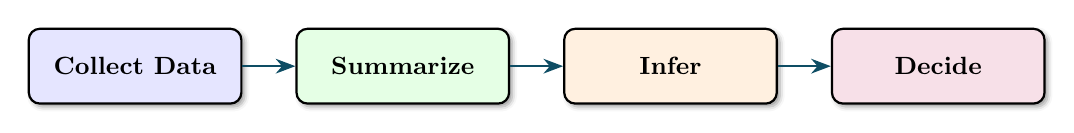
\begin{tikzpicture}[
  nodebox/.style={rectangle, draw, thick, rounded corners=4pt, minimum width=2.7cm, minimum height=0.95cm, align=center, font=\small\bfseries,
    blur shadow={shadow blur steps=3, shadow xshift=0.4mm, shadow yshift=-0.4mm}},
  arr/.style={-{Stealth[length=2.5mm]}, thick, primary}
]
  \node[nodebox, fill=blue!10] (collect) at (0,0) {Collect Data};
  \node[nodebox, fill=green!10] (summarize) at (3.4,0) {Summarize};
  \node[nodebox, fill=orange!12] (infer) at (6.8,0) {Infer};
  \node[nodebox, fill=purple!12] (decide) at (10.2,0) {Decide};
  \draw[arr] (collect) -- (summarize);
  \draw[arr] (summarize) -- (infer);
  \draw[arr] (infer) -- (decide);
\end{tikzpicture}
\end{center}

\begin{longtable}{L{3.5cm}L{7.9cm}}
\toprule
\textbf{Statistical Area} & \textbf{Common Data Science Use} \\
\midrule
Descriptive statistics & Understanding averages, spread, and distributions \\
Probability & Modeling uncertainty and randomness \\
Sampling & Working with subsets instead of full populations \\
Estimation & Approximating unknown parameters \\
Hypothesis testing & Checking if observed effects are statistically meaningful \\
\bottomrule
\end{longtable}

%=============================================================
\section{Data, Variables, and Measurement}
%=============================================================

\subsection{Population and Sample}

\begin{definitionbox}[Population and Sample]
A population is the full group we want to study. A sample is a smaller subset taken from that population.
\end{definitionbox}

\begin{examplebox}[Population and Sample Example]
If a university has 2,000 BSIT students, that entire group is the population. If we survey 120 of them about daily study time, those 120 students form the sample.
\end{examplebox}

\subsection{Types of Variables}

\begin{itemize}[leftmargin=*]
  \item \textbf{Categorical variables:} labels or groups, such as gender, device type, or course section.
  \item \textbf{Numerical variables:} numbers, such as age, salary, accuracy, or response time.
\end{itemize}

Numerical variables are often divided into:

\begin{itemize}[leftmargin=*]
  \item \textbf{Discrete:} countable values, such as number of absences.
  \item \textbf{Continuous:} measured values, such as height or CPU temperature.
\end{itemize}

\begin{conceptbox}[Why Variable Type Matters]
The kind of variable determines which chart, summary, and model are appropriate. A pie chart may suit categories, but a histogram is better for continuous measurements.
\end{conceptbox}

\subsection{Scales of Measurement}

\begin{longtable}{L{2.5cm}L{3.3cm}L{5.4cm}}
\toprule
\textbf{Scale} & \textbf{Example} & \textbf{Interpretation} \\
\midrule
Nominal & Browser type & Categories only, no order \\
Ordinal & Satisfaction level & Ordered categories \\
Interval & Temperature in Celsius & Equal gaps, no true zero \\
Ratio & Income, age, weight & Equal gaps and true zero \\
\bottomrule
\end{longtable}

%=============================================================
\section{Descriptive Statistics: Center of Data}
%=============================================================

\subsection{Mean, Median, and Mode}

Suppose the daily study hours for five students are:
\[
2,\ 3,\ 3,\ 4,\ 8
\]

\begin{itemize}[leftmargin=*]
  \item \textbf{Mean:} the average value
  \item \textbf{Median:} the middle value after sorting
  \item \textbf{Mode:} the most frequent value
\end{itemize}

\begin{examplebox}[Center Example]
For the data $2, 3, 3, 4, 8$:
\[
\text{Mean} = \frac{2+3+3+4+8}{5} = \frac{20}{5} = 4
\]
The middle value is
\[
\text{Median} = 3
\]
The most frequent value is
\[
\text{Mode} = 3
\]
\end{examplebox}

\subsection{When the Mean Can Mislead}

The value 8 is much larger than the others, so it pulls the mean upward.

\begin{alertbox}[Outlier Warning]
The mean is sensitive to extreme values. In skewed data, the median often gives a better picture of the typical case.
\end{alertbox}

\subsection{Weighted Mean}

Sometimes values do not contribute equally. Then we use a weighted mean:
\[
\bar{x}_w = \frac{\sum w_ix_i}{\sum w_i}
\]

\begin{examplebox}[Weighted Mean Example]
Suppose a course grade is composed of quiz = 70 and exam = 90, with weights 40\% and 60\%.
\[
\bar{x}_w = \frac{0.4(70) + 0.6(90)}{1.0} = 28 + 54 = 82
\]
The weighted average is 82.
\end{examplebox}

\subsection{Percentiles and Quartiles}

Percentiles show relative position in a dataset.

\begin{itemize}[leftmargin=*]
  \item 25th percentile = first quartile $Q_1$
  \item 50th percentile = median $Q_2$
  \item 75th percentile = third quartile $Q_3$
\end{itemize}

\begin{conceptbox}[Interpretation]
If a student's score is at the 90th percentile, that means the student scored higher than about 90\% of the observed group.
\end{conceptbox}

%=============================================================
\section{Variability: Spread of Data}
%=============================================================

\subsection{Range}

Range is the difference between the largest and smallest value.

\begin{examplebox}[Range Example]
For the data $5, 7, 9, 10$:
\[
\text{Range} = 10 - 5 = 5
\]
\end{examplebox}

\subsection{Variance and Standard Deviation}

Variance measures average squared distance from the mean, and standard deviation is the square root of variance.

For population variance:
\[
\sigma^2 = \frac{\sum (x - \mu)^2}{N}
\]

For sample variance:
\[
s^2 = \frac{\sum (x - \bar{x})^2}{n-1}
\]

\begin{examplebox}[Sample Variance Example]
Consider the sample data: $4, 6, 8$

Step 1: Find the sample mean.
\[
\bar{x} = \frac{4+6+8}{3} = 6
\]

Step 2: Find deviations from the mean.
\[
4-6=-2, \qquad 6-6=0, \qquad 8-6=2
\]

Step 3: Square the deviations.
\[
(-2)^2=4, \qquad 0^2=0, \qquad 2^2=4
\]

Step 4: Use the sample formula.
\[
s^2 = \frac{4+0+4}{3-1} = \frac{8}{2} = 4
\]

Step 5: Standard deviation.
\[
s = \sqrt{4} = 2
\]
\end{examplebox}

\subsection{Interquartile Range}

The interquartile range measures spread in the middle 50\% of the data.
\[
\text{IQR} = Q_3 - Q_1
\]

\begin{conceptbox}[Why IQR Matters]
IQR is less affected by outliers than the full range. This is useful when the dataset is skewed or contains extreme observations.
\end{conceptbox}

\subsection{Z-Score}

A z-score tells us how many standard deviations a value is from the mean.
\[
z = \frac{x - \bar{x}}{s}
\]

\begin{examplebox}[Z-Score Example]
Suppose a student's score is 85, the class mean is 75, and the standard deviation is 5.
\[
z = \frac{85-75}{5} = 2
\]
The score is 2 standard deviations above the mean.
\end{examplebox}

%=============================================================
\section{Probability Foundations}
%=============================================================

\subsection{Basic Probability}

Probability measures how likely an event is.
\[
P(A) = \frac{\text{favorable outcomes}}{\text{total outcomes}}
\]

\begin{examplebox}[Probability Example]
Suppose a dataset contains 12 fraudulent transactions out of 300 total transactions.
\[
P(\text{fraud}) = \frac{12}{300} = 0.04
\]
So the probability of fraud is 4\%.
\end{examplebox}

\subsection{Complement Rule}

The probability that an event does not occur is
\[
P(A^c) = 1 - P(A)
\]

\begin{examplebox}[Complement Example]
If the probability that a user clicks an ad is 0.18, then the probability that the user does not click is
\[
1 - 0.18 = 0.82
\]
\end{examplebox}

\subsection{Conditional Probability}

Conditional probability asks about one event given another event.
\[
P(A \mid B) = \frac{P(A \cap B)}{P(B)}
\]

\begin{examplebox}[Conditional Probability Example]
In a class, 15 students know Python, 9 know both Python and SQL. If one Python student is selected, the probability that the student also knows SQL is
\[
P(\text{SQL} \mid \text{Python}) = \frac{9}{15} = 0.6
\]
\end{examplebox}

\subsection{Expected Value}

Expected value is the long-run average result of a random process.
\[
E(X) = \sum xP(x)
\]

\begin{examplebox}[Expected Value Example]
Suppose a support chatbot resolves a ticket in 1 minute with probability 0.7 and in 4 minutes with probability 0.3.
\[
E(X) = 1(0.7) + 4(0.3) = 0.7 + 1.2 = 1.9
\]
The expected handling time is 1.9 minutes.
\end{examplebox}

%=============================================================
\section{Random Variables and Common Distributions}
%=============================================================

\subsection{Random Variables}

A random variable assigns a numerical value to an outcome of a random process.

\begin{itemize}[leftmargin=*]
  \item \textbf{Discrete random variable:} number of emails received in an hour
  \item \textbf{Continuous random variable:} time taken to download a file
\end{itemize}

\subsection{Bernoulli and Binomial Ideas}

A Bernoulli variable has only two outcomes, often called success and failure.

If we repeat the same Bernoulli process $n$ times, the total number of successes follows a binomial idea.

\begin{examplebox}[Binomial-Style Example]
Suppose the probability that a student answers a question correctly is 0.8. If the student answers 5 questions, the expected number of correct answers is
\[
E(X) = np = 5(0.8) = 4
\]
\end{examplebox}

\subsection{Normal Distribution}

The normal distribution is a symmetric bell-shaped distribution often used to model natural variation.

\begin{conceptbox}[Why Normality Appears Often]
Many real-world measurements cluster around an average with fewer extreme values, making the normal distribution a useful approximation in practice.
\end{conceptbox}

\subsection{Empirical Rule}

For approximately normal data:

\begin{itemize}[leftmargin=*]
  \item about 68\% of values lie within 1 standard deviation of the mean
  \item about 95\% lie within 2 standard deviations
  \item about 99.7\% lie within 3 standard deviations
\end{itemize}

\begin{examplebox}[Empirical Rule Example]
If server response time has mean 200 ms and standard deviation 20 ms, then about 95\% of response times are expected to lie between
\[
200 - 2(20) = 160
\]
and
\[
200 + 2(20) = 240
\]
milliseconds.
\end{examplebox}

%=============================================================
\section{Sampling and Estimation}
%=============================================================

\subsection{Why Sampling Is Necessary}

In many real problems, measuring the full population is too expensive or impossible. Sampling lets us estimate population behavior using a manageable subset.

\subsection{Sample Mean as an Estimator}

The sample mean estimates the population mean:
\[
\bar{x} = \frac{\sum x}{n}
\]

\begin{conceptbox}[Estimator]
An estimator is a rule for approximating an unknown population parameter. For example, the sample mean estimates the population mean.
\end{conceptbox}

\subsection{Bias and Variability}

A good estimator should be:

\begin{itemize}[leftmargin=*]
  \item \textbf{Unbiased:} correct on average
  \item \textbf{Stable:} not too variable from sample to sample
\end{itemize}

\subsection{Standard Error}

The standard error of the sample mean measures how much the sample mean changes from sample to sample.
\[
SE = \frac{s}{\sqrt{n}}
\]

\begin{examplebox}[Standard Error Example]
Suppose a sample has standard deviation $s = 10$ and size $n = 25$.
\[
SE = \frac{10}{\sqrt{25}} = \frac{10}{5} = 2
\]
The estimated standard error is 2.
\end{examplebox}

\subsection{Confidence Interval Idea}

A confidence interval gives a plausible range for an unknown parameter.

For a 95\% confidence interval for a mean, a common form is:
\[
\bar{x} \pm 1.96(SE)
\]

\begin{examplebox}[Confidence Interval Example]
Suppose a sample mean processing time is 50 seconds and the standard error is 2 seconds.
\[
50 \pm 1.96(2) = 50 \pm 3.92
\]
So the interval is approximately
\[
(46.08, 53.92)
\]
This means the population mean is plausibly between 46.08 and 53.92 seconds.
\end{examplebox}

\begin{alertbox}[Interpretation Warning]
A 95\% confidence interval does not mean there is a 95\% probability that the true mean moves around. It means the method produces correct intervals about 95\% of the time in repeated sampling.
\end{alertbox}

%=============================================================
\section{Hypothesis Testing Intuition}
%=============================================================

\subsection{Null and Alternative Hypotheses}

Hypothesis testing begins with two competing statements:

\begin{itemize}[leftmargin=*]
  \item \textbf{Null hypothesis $H_0$:} no effect, no difference, or current assumption is true
  \item \textbf{Alternative hypothesis $H_1$:} an effect or difference exists
\end{itemize}

\begin{examplebox}[A Testing Example]
Suppose a company claims that a new recommendation algorithm increases click-through rate.

\[
H_0: \text{new model does not improve CTR}
\]
\[
H_1: \text{new model improves CTR}
\]
\end{examplebox}

\subsection{P-Value Intuition}

A p-value measures how surprising the observed result would be if the null hypothesis were true.

\begin{conceptbox}[Interpretation]
A small p-value suggests the data is hard to explain under the null hypothesis, which gives evidence against $H_0$.
\end{conceptbox}

\subsection{Decision Rule}

A common significance level is
\[
\alpha = 0.05
\]

If
\[
p \leq 0.05
\]
we often reject the null hypothesis.

\subsection{Type I and Type II Errors}

\begin{itemize}[leftmargin=*]
  \item \textbf{Type I error:} rejecting a true null hypothesis
  \item \textbf{Type II error:} failing to reject a false null hypothesis
\end{itemize}

\begin{alertbox}[Why Errors Matter]
In fraud detection, medicine, cybersecurity, and business experiments, the cost of a false alarm can be very different from the cost of a missed signal.
\end{alertbox}

%=============================================================
\section{Relationships Between Variables}
%=============================================================

\subsection{Covariance}

Covariance describes whether two variables move together.

\begin{itemize}[leftmargin=*]
  \item Positive covariance: both tend to increase together
  \item Negative covariance: one tends to increase while the other decreases
  \item Near zero covariance: weak linear movement together
\end{itemize}

\subsection{Correlation}

Correlation standardizes covariance and lies between $-1$ and $1$.

\begin{itemize}[leftmargin=*]
  \item $r = 1$: perfect positive linear relation
  \item $r = -1$: perfect negative linear relation
  \item $r = 0$: no linear relation
\end{itemize}

\begin{examplebox}[Correlation Interpretation]
If hours studied and exam score have correlation $r = 0.78$, this suggests a strong positive linear relationship. Students who study more tend to score higher, though not perfectly.
\end{examplebox}

\begin{alertbox}[Correlation Is Not Causation]
Two variables can be related without one directly causing the other. A hidden factor may influence both.
\end{alertbox}

%=============================================================
\section{Statistical Thinking in Data Science Practice}
%=============================================================

\subsection{Train/Test Thinking}

When a model performs well on training data but poorly on new data, we may be seeing overfitting. Statistical thinking reminds us to evaluate on unseen samples, not only on the data used to build the model.

\subsection{A/B Testing}

A/B testing compares two alternatives, such as two website designs or two machine learning models.

\begin{examplebox}[A/B Testing Example]
Suppose Version A gets 40 clicks out of 200 visitors, while Version B gets 54 clicks out of 200 visitors.

Click-through rates:
\[
\text{CTR}_A = \frac{40}{200} = 0.20
\]
\[
\text{CTR}_B = \frac{54}{200} = 0.27
\]
Version B has a higher observed CTR, but we still need statistical testing to judge whether the difference is likely real.
\end{examplebox}

\subsection{Why Uncertainty Should Be Reported}

Predictions, averages, and comparisons should ideally be reported with uncertainty measures such as confidence intervals, p-values, or standard errors.

\begin{conceptbox}[Good Reporting Practice]
Instead of saying ``the average response time is 50 seconds,'' a better statement is ``the average response time is about 50 seconds, with a 95\% confidence interval from 46.08 to 53.92 seconds.''
\end{conceptbox}

%=============================================================
\section{Quick Reference Summary}
%=============================================================

\begin{longtable}{L{3.6cm}L{7.6cm}}
\toprule
\textbf{Concept} & \textbf{Key Formula or Idea} \\
\midrule
Mean & $\bar{x} = \frac{\sum x}{n}$ \\
Weighted mean & $\bar{x}_w = \frac{\sum w_ix_i}{\sum w_i}$ \\
Range & $\max(x) - \min(x)$ \\
Sample variance & $s^2 = \frac{\sum (x-\bar{x})^2}{n-1}$ \\
Standard deviation & $s = \sqrt{s^2}$ \\
Z-score & $z = \frac{x-\bar{x}}{s}$ \\
Probability & $P(A) = \frac{\text{favorable}}{\text{total}}$ \\
Conditional probability & $P(A \mid B) = \frac{P(A \cap B)}{P(B)}$ \\
Expected value & $E(X) = \sum xP(x)$ \\
Standard error & $SE = \frac{s}{\sqrt{n}}$ \\
Confidence interval & estimate $\pm$ margin of error \\
\bottomrule
\end{longtable}

%=============================================================
\section{Key Takeaways and Review Questions}
%=============================================================

\subsection{Key Takeaways}

\begin{itemize}[leftmargin=*]
  \item Statistics helps turn raw data into meaningful evidence.
  \item Measures of center describe typical values.
  \item Measures of spread describe consistency and variation.
  \item Probability gives a formal way to reason about uncertainty.
  \item Sampling and estimation let us study populations efficiently.
  \item Hypothesis testing supports evidence-based decisions.
\end{itemize}

\subsection{Review Questions}

\begin{enumerate}[leftmargin=*]
  \item What is the difference between a population and a sample?
  \item When is the median more useful than the mean?
  \item How do variance and standard deviation differ?
  \item What does a z-score tell us?
  \item Why is conditional probability useful in data science?
  \item What is the role of a confidence interval?
  \item Why does correlation not automatically imply causation?
\end{enumerate}

\begin{examplebox}[Short Reflection Task]
Collect a small dataset from daily life, such as quiz scores, internet speed tests, or daily expenses. Compute the mean, median, range, and standard deviation. Then explain what these summaries reveal about the data.
\end{examplebox}

\vfill
\begin{center}
{\large\textcolor{primary}{\textbf{End of Handout}}}\\[4pt]
{\small\textcolor{gray!70!black}{Statistical Foundations of Data Science --- BSIT Program}}
\end{center}

\end{document}